\chapter{Design Overview}

\section{Introduction}
The Design Overview is section to introduce and give a brief overview of the design.  The System
Architecture is a way to give the overall view of a system and to place it into context with external
systems.  This allows for the reader and user of the document to orient them selves to the design and
see a summary before proceeding into the details of the design.

\section{System Architecture}
\begin{figure}[H]
\centering
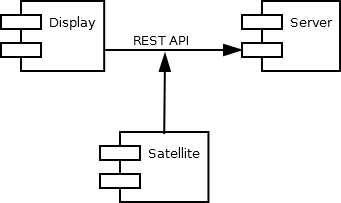
\includegraphics[scale=0.7]{Software/images/SystemOverviewDiagram.png}
\caption{System Overview}
\label{SystemOverview}
\end{figure}

\section{Assumptions}
It is assumed that an entire system consists of one Server, and one or more Satellites.